
\begin{definition}[Plano axial:] 
\index{Plano axial}
\label{def:PlanoAxial}
O Dicionário Priberam da Língua Portuguesa \cite{priberamplano} define plano axial como:
Plano transversal, plano horizontal que divide o corpo ou uma estrutura anatômica em parte superior e parte inferior.
Ver Figura \ref{fig:bodyhumanplane}.
\end{definition}

\begin{definition}[Plano frontal:] 
\index{Plano frontal}
\label{def:PlanoFrontal}
O Dicionário Priberam da Língua Portuguesa \cite{priberamplano} define plano frontal como:
Plano coronal,   plano vertical e paralelo à sutura coronal do crânio, que divide o corpo em parte anterior e parte posterior.
Ver Figura \ref{fig:bodyhumanplane}.
\end{definition}

\begin{definition}[Plano sagital:] 
\index{Plano sagital}
\label{def:PlanoSagital}
O Dicionário Priberam da Língua Portuguesa \cite{priberamplano} define plano sagital como:
Plano vertical e paralelo à sutura sagital do crânio, que divide o corpo em parte direita e parte esquerda.
Ver Figura \ref{fig:bodyhumanplane}.
\end{definition}

\begin{figure}[h!]
  \centering
    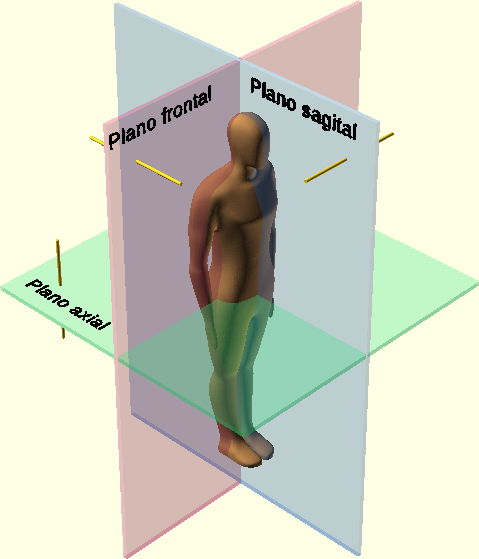
\includegraphics[width=0.60\textwidth]{body-plane/files/body-plane.png}
  \caption{ Planos e eixos no corpo humano.}
\label{fig:bodyhumanplane}
\end{figure}

\begin{definition}[Eixo axial:] 
\index{Eixo axial}
\label{def:EixoAxial}
É o eixo perpendicular ao plano axial.
Ver Figura \ref{fig:bodyhumanplane}.
\end{definition}

\begin{definition}[Eixo frontal:] 
\index{Eixo frontal}
\label{def:EixoFrontal}
É o eixo perpendicular ao plano frontal.
Ver Figura \ref{fig:bodyhumanplane}.
\end{definition}

\begin{definition}[Eixo sagital:] 
\index{Eixo sagital}
\label{def:EixoSagital}
É o eixo perpendicular ao plano sagital.
Ver Figura \ref{fig:bodyhumanplane}.
\end{definition}

\begin{definition}[Passo cíclico:] 
\index{Passo cíclico}
\label{def:PassoCiclico}
É um passo de dança que pode acontecer por um tempo indeterminado,
devido a que este está composto por ciclos, cuja postura de inicio e final é a mesma.
\end{definition}

\begin{definition}[Passo simétrico:] 
\index{Passo simétrico}
\label{def:PassoSimetrico}
É um passo de dança que tem a primeira metade do passo similar à segunda,
com a diferencia que se executa com os pés intercambiado (direita por esquerda)
ou com as posições dos corpos intercambiadas (seguidor por condutor).
\end{definition}

\begin{definition}[Duração do movimento:] 
\index{Duração do movimento}
\label{def:DuracaoDoPasso}
Ou a \textbf{duração do passo}, 
é a longitude temporal de um passo de dança, contado em tempos da música.
No caso de \hyperref[def:PassoCiclico]{\textbf{passos cíclicos}}, a duração do passo se refere a duração do ciclo.
\end{definition}


\begin{definition}[Dançar no tempo forte:] 
\index{Dançar no tempo forte}
\label{def:DancaNoTempo}
Ou simplesmente \textbf{dançar no tempo}, indica que se está dançando com passos com o movimento principal ou inicial (dependendo do estilo de dança), 
se executando no tempo forte da música; ver Exemplo \ref{example:dancatempoforte}.
\end{definition}
\begin{example}
\label{example:dancatempoforte}
Se definimos um passo de dança como: Pisar, usando um pé cada vez, 
realizando um movimento com uma distribuição espacial, junto-junto-longo;
e definimos ao movimento ``longo'' como o movimento principal. 
Se executássemos o movimento ``longo'' no tempo forte, o passo junto-junto-longo,
estaria sendo dançado no tempo forte.
\end{example}

\begin{definition}[Dançar em contratempo:] 
\index{Dançar no contratempo}
\label{def:DancaNoContratempo}
Indica que se está dançando, com o movimento principal ou inicial (dependendo do estilo de dança) do passo, 
executando-se em contra do tempo forte da música; é dizer, executando-se num tempo fraco (em contratempo).
Com diferencia de \hyperref[def:DancaNoTempo]{\textbf{dançar no tempo forte}}, 
que é único, pois só existe um tempo forte;
existem varias formas de dançar como o movimento principal em algum tempo fraco; ver Exemplo \ref{example:dancatempofraco}.
\end{definition}
\begin{example}
\label{example:dancatempofraco}
Se definimos um passo de dança como: Pisar, usando um pé cada vez, 
realizando um movimento com uma distribuição espacial, junto-junto-longo;
e definimos ao primeiro movimento ``junto'' como o movimento principal. 
Se executássemos o movimento ``longo'' no tempo forte, o passo junto-junto-longo,
estaria sendo dançado em contratempo.
\end{example}

\begin{definition}[Passo a contratempo:] 
\index{Passo a contratempo}
\label{def:PassoAContratempo}
É um passo de dança cuja execução promove que quando se esteja dançando com um pé especifico acompanhando o tempo forte da música,
ao finalizar o passo este pé esteja sendo marcado no tempo fraco.
É dizer, são movimento onde após de realizados, 
passamos de \hyperref[def:DancaNoTempo]{\textbf{dançar no tempo}} a 
\hyperref[def:DancaNoContratempo]{\textbf{dançar no contratempo}} e vice-versa. 
No samba de gafieira, isto acontece quando o número de tempos musicais que o passo  usa é impar;
pois as músicas tradicionalmente são escritas sombre compassos binários, 
pelo que comumente acharemos um tempo forte intercalado por uno tempo fraco.
\end{definition}

\begin{definition}[Passo de deslocamento:] 
\index{Passo de deslocamento}
\label{def:PassoDeDeslocamento}
É um passo de dança cujo propósito, consequência ou objetivo é o deslocamento no salão.
\end{definition}

\begin{definition}[Postura de finalização:] 
\index{Postura, tipos!Postura de finalização}
\label{def:PosturaFinaliza}
É uma postura a qual da a percepção, 
de que se tem chegado ao ponto final da ideia expressada com o movimento.
Se nossa dança fosse um relato escrito, esta postura seria equivalente a um ponto ou ponto e virgula.
\end{definition}

\begin{definition}[Postura de transição:] 
\index{Postura, tipos!Postura de transição}
\label{def:PosturaTransicao}
É uma postura a qual da a percepção, 
de que não se tem completado a ideia expressada com o movimento, e que possivelmente vem mais algum outro movimento.
Se nossa dança fosse um relato escrito, esta postura seria equivalente a uma virgula ou espaço em branco entre as palavras.
\end{definition}

